\chapter{Projekt, etap I -- Badanie (Exploration)}
\label{cha:EtapI}

Zgodnie z cyklem życia ,,XP'' (więcej \namedref{sec:ZMTOcykl}), projekt zaczyna się od akwizycji ogólnego, głównego zadania systemu. Proponuje się w tym celu wykorzystać przygotowany szablon (więcej \namedref{sec:dodatekAsgzs}). Zawiera on nie tylko najważniejszą część, czyli ogólny opis głównego zadania systemu, ale także szereg pomocnych pytań pomagających w realizacji systemu zgodnie z oczekiwaniami klienta. Szablonu nie należy traktować jako idealnego, a raczej jako propozycję lub punkt wyjścia do rozwinięcia własnego dokumentu wykorzystywanego do akwizycji ogólnych wymagań w swoich projektach.

Sformułowanie głównego zadania systemu pozwala skupić się generowaniu kart wymagań związanych z~nim, a~nie ze~sprawami pobocznymi. Pozwala na uzmysłowienie grupie projektowej jaka jest główna część systemu wokół której należy się skupić.

\section{Specyfikacja wymagań}
\label{sec:EtapIsw}

\subsection{Specyfikacja głównego zadania systemu}
\label{sec:EtapIswSGZS}

Niżej przedstawiono szablon (więcej \namedref{sec:dodatekAsgzs}) wypełniony razem z klientem na jednym z pierwszych spotkań dotyczących wymagań systemu.

\begin{userstory}{Główne zadanie systemu}
Użytkownik za pomocą smartphone'a z kamerą działającego pod systemem Android lub za pomocą przeglądarki internetowej na komputerze stacjonarnym i kamery podłączonej do niego, ma możliwość udostępnienia on-line aktualnego obrazu i dźwięku.
    \begin{questions}
        \item{
            \textbf{Kto jest użytkownikiem systemu?} Użytkownikiem systemu może być każdy kto ma przeglądarkę. Aby udostępnić swoją kamerę dodatkowo użytkownik musi być zalogowany, a wcześniej zarejestrowany w systemie. Aby korzystać z reszty funkcji serwisu nie trzeba być zalogowanym.
        }
        \item{
            \textbf{Jakie urządzenia muszą współpracować z systemem?} Wszystkie komputery wyposażone w przeglądarkę IE 7.0+, Firefox 3+, Chrome, Opera 9+. Dodatkowo system ma działać na telefonach komórkowych / tabletach z systemem Android.
        }
        \item{
            \textbf{Czy jest wymóg użycia konkretnej technologii?} Nie jest wymagana żadna konkretna technologia. Wymaganiem jest wykorzystanie technologii Open Source -- wszędzie tam gdzie jesteśmy w stanie zastąpić komercyjne rozwiązania.
        }
        \item{
            \textbf{Jaka jest wymagana skalowalność systemu?} System musi być skalowalny, idealnie by było, gdyby obraz z kamery udostępniany przez jednego użytkownika, mógłby być odbierany przez nieskończoną liczbę ludzi. Na pewno w jakiś sposób system musi reagować automatycznie na zwiększony ruch w obrębie jednego stream'a.
        }
        \item{
            \textbf{Czy są jakieś wymagania dotyczące środowiska produkcyjnego w jakim ma działać system?} System docelowo będzie wdrożony na odpowiednim sprzęcie, testy powinien być w stanie odpalić się na średniej klasy laptopie. Im mniejsze wymagania tym lepiej.
        }
        \item{
            \textbf{Czy system ma współpracować z innymi systemami lub udostępniać coś innym systemom?} Duży nacisk będzie kładziony na integrację z serwisami społecznościowymi, głównie chodzi o Facebook'a. Będzie można go wykorzystać celem rejestracji i logowania w serwisie, czy też automatycznego udostępniania stream'u na swojej Facebook'owej ścianie.
        }
        \item{
            \textbf{Czy istnieją systemy podobne do tworzonego?} Jeżeli chodzi o sposób prezentacji interfejsu WWW to najbardziej zbliżony do tego co chce się osiągnąć jest Bambuser. Podobnie ma się sprawa funkcjonalności na telefonie z systemem Android -- aplikacja Bambuser.
        }
        \item{
            \textbf{Czy są jakieś inne specjalne wymagania, które nie wynikają z funkcji jakie powinien posiadać system (wymagania niefunkcjonalne)?} Szybki, skalowalny, bezpieczny, wykorzystujący technologie Open Source.
        }
    \end{questions}
\end{userstory}

\subsection{Karty wymagań dla ,,pierwszego wydania''}
\label{sec:EtapIswKWDPW}

Akwizycja głównego zadania systemu pozwala na przejście do kolejnego etapu, w którym przygotowuje się wszystkie karty wymagań dla ,,pierwszego wydania'' (więcej \namedref{sec:ZMTOcykl}). Faza ta trwa do momentu kiedy klient nie będzie już miał pomysłu na karty wymagań związane z głównym zadaniem systemu lub grupa projektowa nie będzie w stanie lepiej oszacować czasu potrzebnego na wykonanie danej karty wymagań bez rozpoczęcia jej implementacji.

\begin{userstory}{Strona główna dla niezalogowanego użytkownika}
    Użytkownikowi niezalogowanemu w systemie, po wejściu na główną domenę serwisu, zostaje zaprezentowana zawartość w postaci:
    \scr{img/strona_glowna.jpg}{Strona główna dla niezalogowanego użytkownika}
    \begin{packed_enum}
        \item odnośnik przekierowujący zawsze na stronę główną serwisu
        \item wyszukiwarka umożliwiająca wyszukiwanie udostępnionych streamów audio/video po kategoriach i lokalizacji
        \item dwa odnośniki, dzięki którym pokazuje się formularz logowania lub rejestracji
        \item mapa pokazująca grupy streamów audio/wideo
    \end{packed_enum}

    \begin{tests}
        \item{
            Użytkownik po wejściu na stronie główną widzi mapę swojej okolicy (fizycznej lokalizacji). Lokalizację możemy oszacować za pomocą IP lub jak jest taka możliwość w każdy inny dokładniejszy sposób.
        }
        \item{
            Użytkownik może dowolnie przesuwać mapą. Mapa reaguje na przesuwanie, oraz są na niej aktualizowane punkty streamów audio/video.
        }
    \end{tests}
\end{userstory}

\begin{userstory}{Strona główna dla zalogowanego użytkownika}
    Użytkownikowi zalogowanemu w systemie, po wejściu na główną domenę serwisu, zostaje zaprezentowana zawartość w postaci:
    \scr{img/strona_glowna2.jpg}{Strona główna dla zalogowanego użytkownika}
    \begin{packed_enum}
        \item avatar pobrany z gravatar.com oraz nazwa zalogowanego użytkownika
        \item wpis w menu przenoszący do podstrony ustawień zalogowanego użytkownika
        \item wpis w menu przenoszący do podstrony udostępniania streamu audio/video
    \end{packed_enum}
    \begin{tests}
        \item{
            Po kliknięciu w menu na pozycję z nazwą zalogowanego użytkownika, pojawiają się poniższe wpisy w menu.
        }
    \end{tests}
\end{userstory}

\begin{userstory}{Rejestracja}
    Użytkownik po naciśnięciu odnośnika rejestruj,
    zostaje przekierowany do formularza rejestracji:
    \scr{img/rejestracja.jpg}{Formularz rejestracji.}
    \begin{tests}
        \item{
            Pole email i powtórz email muszą być takie same, inaczej wyświetlany jest błąd, użytkownik proszony jest o poprawę pól.
        }
        \item{
            Pole hasło i powtórz hasło muszą być takie same, inaczej wyświetlany jest błąd, użytkownik proszony jest o poprawę pól.
        }
        \item{
            Pole loginu musi być unikalne w bazie. W przypadku wystąpienia w bazie zwracamy użytkownikowi błąd.
        }
        \item{
            Pole email musi być unikalne w bazie. W przypadku wystąpienia w bazie zwracamy użytkownikowi błąd.
        }
        \item{
            Po prawidłowym wypełnieniu formularza, użytkownik dostaje informację o konieczności potwierdzenia swojego adresu e-mail. Aby potwierdzić rejestrację musi kliknąć w link aktywacyjny wysłany na rejestrowane konto pocztowe, w ciągu 7 dni od momentu rejestracji. W innym wypadku konto nie zostanie aktywowane, a zgłoszenie usunięte z bazy.
        }
    \end{tests}
\end{userstory}

\begin{userstory}{Przypomnienie hasła}
    Użytkownik po naciśnięciu odnośnika zapomniałem hasła,
    zostaje przekierowany do formularza przypomnienia hasła:
    \scr{img/przypomnenie_hasla.jpg}{Formularz przypomnienia hasła.}
    \begin{tests}
        \item{
            Po wpisaniu istniejącego loginu lub maila, na maila wysyłane jest zapytanie, czy chcemy resetować hasło z linkiem aktywującym. Po jego kliknięciu otrzymujemy drugi mail z wygenerowanym nowym hasłem, które później możemy zmienić na zakładce ,,Ustawienia''.
        }
        \item{
            Użytkownik po podaniu błędnego loginu/maila zostaje o tym poinformowany ekranem:
            \scr{img/przypomnenie_hasla2.jpg}{Ekran informacji o błędnym wypełnieniu loginu/hasła.}
        }
    \end{tests}
\end{userstory}

\begin{userstory}{Logowanie użytkownika}
    Użytkownik po naciśnięciu odnośnika zaloguj,
    zostaje przekierowany do formularza logowania:
    \scr{img/logowanie.jpg}{Formularz logowania.}
    \begin{packed_enum}
        \item reszta strony wyszarzona, formularz logowania jako ,,overlay''
        \item klikając X'a wracamy do wyszarzonej strony
        \item miejsce na wpisanie loginu lub email
        \item miejsce na wpisanie hasła
        \item link do formularza przypomnienia hasła
        \item przycisk wysyłający formularz logowania
    \end{packed_enum}
    
    \begin{tests}
        \item{
            Użytkownik tylko po podaniu istniejącego loginu oraz pasującego do niego hasła
            zostaje zalogowany i przeniesiony na oglądaną przed logowaniem stronę.
        }
        \item{
            Użytkownik po zalogowaniu ma dostęp do dodatkowych podstron -- Ustawienia, Podziel się!
        }
        \item{
            Użytkownik po podaniu błędnego hasła lub nieistniejącego loginu, zostaje o tym poinformowany ekranem:
            \scr{img/logowanie2.jpg}{Ekran informacji o błędnym haśle lub loginie.}
            \begin{packed_enum}
                \item informacja o typie błędu
                \item oznaczenie pól jako błędnie wypełnionych, pole hasła pozostaje puste, pole loginu zostaje jako ostatnia wpisana wartość
            \end{packed_enum}
        }
        \item{Użytkownik po zalogowaniu widzi zmodyfikowane menu -- na wszystkich podstronach serwisu.}
        \scr{img/strona_glowna2.jpg}{Zmodyfikowane menu na górze}
    \end{tests}
\end{userstory}

\begin{userstory}{Udostępnianie streamu audio/video krok pierwszy}
    Użytkownik po wybraniu z menu opcji podziel się,
    zostaje przekierowany do formularza udostępniania audio/video:
    \scr{img/dzielenie_sie_streamem1.jpg}{Formularz udostępniania audio/video.}
    \begin{packed_enum}
        \item {Aby udostępnić stream należy wybrać kategorię, do której ten stream ma być przypisany. Lista kategorii jest przykładową lista, administrator ma mieć możliwość modyfikowania tej listy z poziomu panelu administracyjnego.}
        \item {Jeżeli w systemie istnieje więcej niż jedna kamera, tutaj wybierana jest kamera źródłowa. Domyślnie wybraną jest pierwsza systemowa kamera.}
        \item {Możemy wybrać jakość transmisji spośród:
            \begin{packed_item}
                \item{wysoka -- wysoka jakość z preferencją wideo nad audio}
                \item{średnia -- średnia jakość zarówno wideo jak audio}
                \item{niska -- niska jakość wideo z preferencją jakości audio nad wideo}
            \end{packed_item}
        }
        \item{Po kliknięciu ,,Podziel się'' na formularzu udostępniania audio/video, użytkownikowi otwiera się nowe okno przeglądarki gdzie prezentowane są dane udostępnionego streamu (krok drugi). W starym oknie użytkownik zostaje przekierowany do poprzednio odwiedzanej strony -- przed wybraniem ,,Podziel się''.}
        \item {Wybór dostępności streamu, albo publiczny -- wszyscy użytkownicy systemu mogą go oglądać/udostępniać (domyślna opcja) -- lub prywatny -- tylko posiadający link do streamu mogą go zobaczyć.}
    \end{packed_enum}
    \begin{tests}
        \item{Jeżeli w systemie nie ma kamery, użytkownik jest informowany o braku możliwości udostępniania, przycisk ,,Podziel się!'' staje się nieaktywny.}
    \end{tests}
\end{userstory}

\begin{userstory}{Udostępnianie streamu audio/video krok drugi}
    Po kliknięciu ,,Podziel się'' na formularzu udostępniania audio/video, użytkownikowi otwiera się nowe okno przeglądarki gdzie prezentowane są dane udostępnionego streamu. W starym oknie użytkownik zostaje przekierowany do poprzednio odwiedzanej strony -- przed wybraniem ,,Podziel się''.
    \scr{img/dzielenie_sie_streamem2.jpg}{Okno danych udostępnianego streamu audio/video.}
    \begin{packed_enum}
        \item{możliwość zmiany kamery oraz jakości w trakcie nadawania}
        \item{jeżeli wcześniej wybrano publiczną dostępność streamu, wyświetlamy tutaj unikalny link do dzielenia się streamem ze znajomymi np. za pomocą Facebook'a, w przeciwnym wypadku wyświetlamy ,,permalink'' streamu w formie \url{http://domena.com/login_usera/slug_tytulu_streamu}}
        \item{przycisk otwierający w nowym oknie link streamu}
        \item{informacja na temat tytułu oraz kategorii udostępnianego streamu}
    \end{packed_enum}
    \begin{tests}
        \item{Po kliknięciu na pole tekstowe linku, zaznacza się cała zawartość. Dodatkowo zaznaczona zawartość zostaje skopiowana do schowka, na ekranie pojawia się informacja ,,Link skopiowano do schowka!''}
    \end{tests}
\end{userstory}

\section{Analiza wymagań}
\label{sec:EtapIaw}

Po rozmowie z klientem, na podstawie ,,głównego zadania systemu'' oraz innych przygotowanych kart wymagań, można przejść do fazy analizy wymagań (więcej w \namedref{sec:ZMTOzwinnaAnalizaWymagan}).

Zgodnie z założeniami ,,XP'' (więcej \namedref{sec:ZMTOzalozenia}), wszystkie ustalenia sporządzone w tej fazie mogą ulec zmianie na każdym późniejszym etapie prowadzenia projektu. Zwinna analiza wymagań nie zamyka możliwości późniejszej zmiany technologii, architektury czy dowolnego z elementów wspomagających projekt.

Celem tego etapu jest stworzenie wstępnej architektury systemu, przetestowanie wydajności technologii -- najczęściej przy użyciu prototypu systemu.

Jako początek rozważań architektury systemu skorzystano z elementów metody Architecture Tradeoff Analysis Method -- ,,Drzewo użyteczności'' oraz ,,Ryzyka i nie ryzyka'' -- szczegóły metody można poznać w \cite{Kaz2000}.

Pełna metoda ATAM wprowadza zbyt dużą formalizację i generuje zbyt dużą ilość dokumentacji, z której metodyki zwinne chcą rezygnować (\namedref{sec:ZMTOzalozenia}).

\subsection{Drzewo użyteczności (ATAM Usability Tree)}
\label{sec:EtapIdrzewoUzytecznosci}

\begin{packed_item}
    \item{
        \textbf{WYDAJNOŚĆ}
        \begin{packed_item}
            \item{
                Opóźnienie transmisji danych
                \begin{packed_item}
                    \item{opóźnienie wideo dostosowane do aktualnej przepustowości łącza, jak najmniejsze}
                    \item{brak lub minimalne opóźnienia transmisji audio}
                \end{packed_item}
            }
            \item{
                Ilość użytkowników
                \begin{packed_item}
                    \item{Liniowa zależność ilość użytkowników używających system od zużywanych zasobów}
                    \item{Minimalna ilość użytkowników aktywnie poruszających się po stronie -- 1000 osób}
                    \item{Minimalna ilość użytkowników oglądających jeden strumień wideo -- 100 osób}
                \end{packed_item}
            }
        \end{packed_item}
    }
    \item{
        \textbf{MODYFIKOWALNOŚĆ}
        \begin{packed_item}
            \item{Zarządzanie użytkownikami}
            \item{Zarządzanie dostępnymi streamami}
            \item{Zarządzanie kategoriami streamów}
            \item{Aktualizacja i dystrybucja oprogramowania mobilnego}
            \item{Łatwa modyfikacja wyglądu strony}
        \end{packed_item}
    }
    \item{
        \textbf{DOSTĘPNOŚĆ}
        \begin{packed_item}
            \item{Dostępność całej usługi na poziomie 99,9\% rocznie}
            \item{Dostępność usługi na urządzenia mobilne (tablety, telefony)}
            \item{Dostępność usługi na desktopy}
        \end{packed_item}
    }
    \item{
        \textbf{SKALOWALNOŚĆ}
        \begin{packed_item}
            \item{Odporność na geometryczną ,,nagłą popularyzację''}
            \item{Liniowa zależność ilość użytkowników/zużywane zasoby}
        \end{packed_item}
    }
    \item{
        \textbf{BEZPIECZEŃSTWO}
        \begin{packed_item}
            \item{
                System logowania
            }
            \item{
                Stream publiczny/prywatny
            }
            \item{
                Szyfrowanie
                \begin{packed_item}
                    \item{wymagane szyfrowanie transmisji wideo}
                    \item{wymagane szyfrowanie transmisji audio}
                    \item{wymagane szyfrowanie transmisji http i każdej innej transmisji danych poza system}
                \end{packed_item}
            }
        \end{packed_item}
    }
\end{packed_item}

\subsection{Wstępna architektura systemu}

Docelowy system będzie się składał z \textbf{Interfejsu WWW}, odpowiedzialnego za prezentację mapy i dostosowywanie się do zmiennej szerokości ekranu urządzeń. Wszystkie stream'y będą umieszczone w relacyjnej \textbf{Bazie danych} z rozszerzeniem GIS, dzięki czemu możliwe będzie łatwe zapisanie lokalizacji stream'u.

Po stronie komputerów stacjonarnych, za pobieranie obrazu z kamery i wyświetlanie obrazu u drugiego użytkownika będzie odpowiedzialny obiekt SWF \textbf{Adobe Flash Player}. W przypadku urządzeń mobilnych, do przygotowania aplikacji obsługującej zarówno iPhone'a jak i Androida wykorzystany zostanie otwarty framework Adobe Flex i jego mobilne wsparcie w postaci \textbf{Adobe AIR for Mobile}.

Do rozproszenia ruchu i stworzenia systemu niezależnego od pojedynczego punktu połączenia sieciowego -- osoby udostępniającej stream -- będą wykorzystane sieci ze wspomaganiem równorzędnym wbudowane w Adobe Flash Platform. Zasada działania sieci P2P, wymusza udostępnianie oglądanego streamu, tak aby zapewnić prostą zależność -- im więcej użytkowników chce oglądać, tym więcej użytkowników udostępnia żądany stream. Firma Adobe nazywa tę technologię \textbf{Multicast/P2P Multicast}, niżej przedstawione są schematy pokazujące różnicę pomiędzy transmisją Unicast, a P2P Multicast. \footnote{informacje dotyczące technologii Adobe oraz obrazki zostały pobrane z \cite{TomKrcha2010ME} oraz \cite{KevinTow2010}}

\begin{center}
    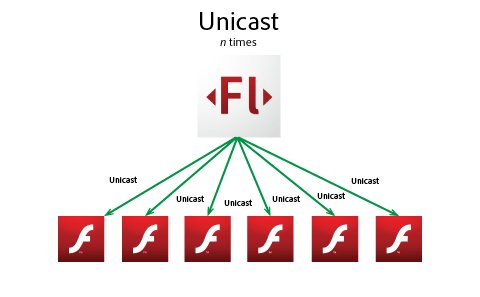
\includegraphics[width=\textwidth]{img/adobe-p2p-unicast.jpg}
    \captionof{figure}{Adobe Flash Platform Unicast -- wszystko zależne od przepustowości jednego elementu źródłowego, serwera plików}
\end{center}

\begin{center}
    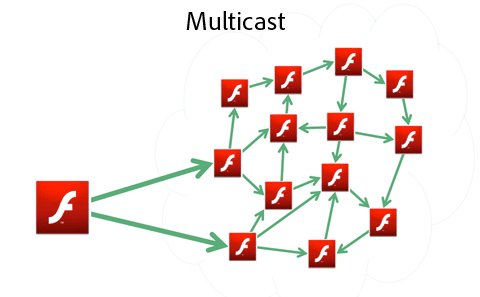
\includegraphics[width=\textwidth]{img/adobe-p2p-multicast.jpg}
    \captionof{figure}{Adobe Flash Platform P2P Multicast -- obciążenie rozłożone na całość sieci ze wspomaganiem równorzędnym}
\end{center}

\newpage
Jako, że technologie, które zostaną wykorzystane są nowe dla całej ,,grupy projektowej'', będzie potrzebny prototyp systemu. Niżej przedstawiono schematy pokazujące powiązanie pomiędzy poszczególnymi elementami systemu:

\begin{center}
    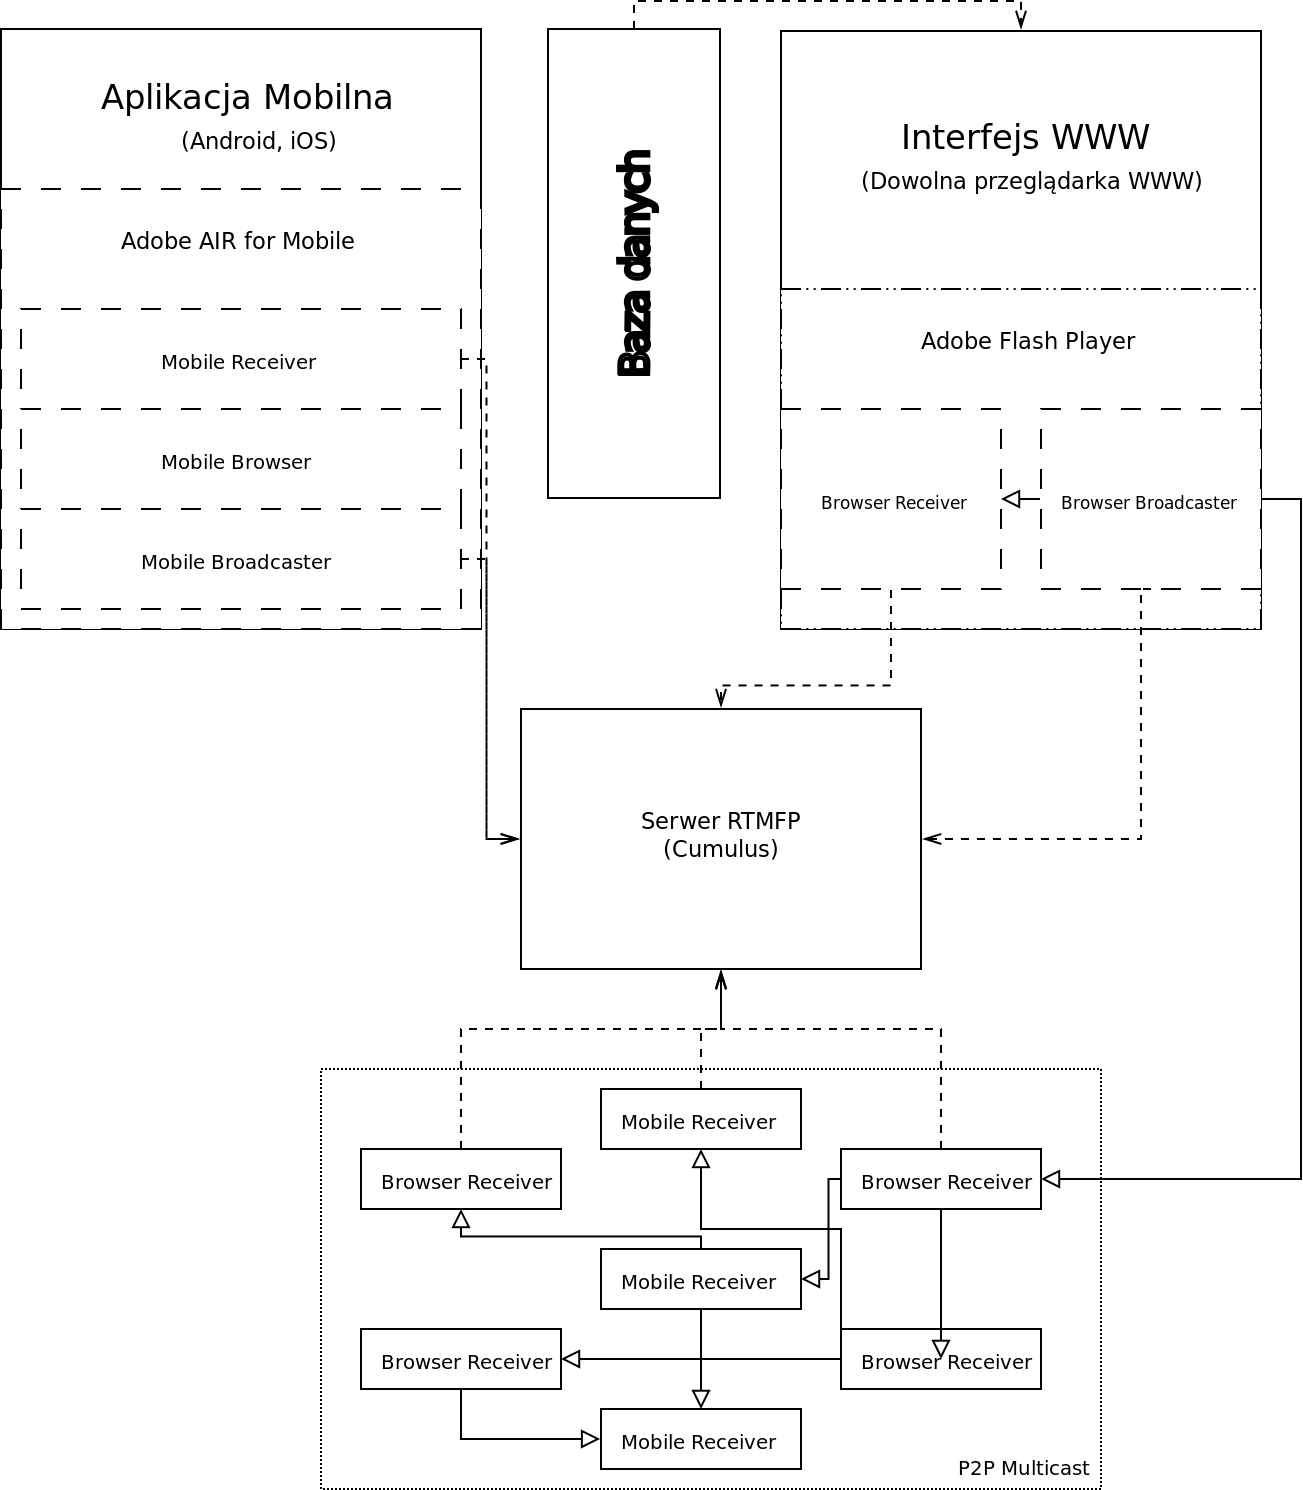
\includegraphics[width=\textwidth]{diagramy/architektura.png}
    \captionof{figure}{Wstępna architektura systemu.}
\end{center}

\subsection{Technologia}
\subsection{Ryzyka/wrażliwości systemu}
% - Architektura (tutaj coś o ATAM i uzasadnienie dlaczego tylko ograniczam się do 2 elementów)
%-- Usability Tree
%-- Proponowana architektura systemu (dekompozycja na screenshotach + opis)
%-- Technologie (tutaj opis dlaczego akurat te - powiązanie z specyfikacją wymagań)
%-- Ryzyka/wrażliwości systemu z taką architekturą i taką technologią
\newpage
%---------------------------------------------------------------------------
